\documentclass[11pt,a4paper]{ctexart}
\usepackage[teacher]{../../ipara}
\usepackage{mathtools}
\usepackage{amsthm}
\newtheorem{theorem}{定理}
\usepackage{longtable}
\usepackage{booktabs}
\raggedbottom

\pagestyle{fancy}
\fancyhf{}
\lhead{\small 专题讲义：极值点偏移的本质与母模型体系}
\rhead{\small 数学一对一}
\cfoot{\small 第 \thepage\ 页\quad 共 \pageref{LastPage} 页}
\renewcommand{\headrulewidth}{0.4pt}
\renewcommand{\footrulewidth}{0pt}

\newcommand{\lessoninfo}[2]{%
  \begin{center}
    {\LARGE\bfseries #1 \quad (教师/学案兼用版)}\par
    \vspace{0.8em}
    {\small 适用：#2}
  \end{center}
  \vspace{0.6em}
  \rule{\linewidth}{0.5pt}
}

% 引入一些数学运算符
\providecommand{\csch}{\operatorname{csch}}

\begin{document}

\lessoninfo{极值点偏移的本质与母模型体系}{高二/高三压轴突破、强基计划}

\section{什么是极值点偏移}

\begin{teachbox}{现象引入}
“极值点偏移”不是一个固定定理名，更像是一类题的现象和方法。

它研究的是：$f(x_1)=f(x_2)$，其中 $x_1<x_0<x_2$，且 $x_0$ 是函数的极值点。因为 $x_1,x_2$ 在极值点两侧，函数值相等，所以它们像是关于极值点“对称”的两个点。但很多函数并不真正对称，于是会出现：
\[
x_1+x_2>2x_0 \quad \text{或者} \quad x_1+x_2<2x_0
\]
或者在正数区间更常见：
\[
x_1x_2>x_0^2 \quad \text{或者} \quad x_1x_2<x_0^2
\]
这种“看起来应该对称，但实际上偏向一侧”的现象，就叫\textbf{极值点偏移}。
\end{teachbox}

\subsection{存在唯一性的铺垫（以 $x-\ln x$ 为例）}
对 $f(x)=x-\ln x$ ($x>0$)，有
\[
f'(x)=1-\frac{1}{x}=\frac{x-1}{x}.
\]
so $f(x)$ 在 $(0,1)$ 上单调递减，在 $(1,+\infty)$ 上单调递增，且 $f(1)=1$。

又因为
\[
\lim_{x\to 0^+}(x-\ln x)=+\infty,\qquad
\lim_{x\to +\infty}(x-\ln x)=+\infty,
\]
且 $f(1)=1$，所以当 $m>1$ 时，方程 $x-\ln x=m$ 在 $(0,1)$ 上至少有一根，在 $(1,+\infty)$ 上至少有一根。
结合 $f(x)$ 在 $(0,1)$ 上严格递减、在 $(1,+\infty)$ 上严格递增，可知两根唯一，分别记为 $x_1, x_2$，且必然有
\[
x_1<1<x_2.
\]
这是后续所有偏移讨论的合法性来源与讨论前提。

\section{极值点不是对称轴}
学生最容易误以为：$f(x_1)=f(x_2)$，且 $x_1<x_0<x_2$ 就应该有 $x_1+x_2=2x_0$。但这只在函数关于 $x=x_0$ 对称时才成立。极值点只是告诉我们：左边一支、右边一支，可以被同一条水平线截出两个点。
\[
\boxed{\text{有极值点，只说明有“两侧等高”；不说明“两侧等距”。}}
\]

\begin{center}
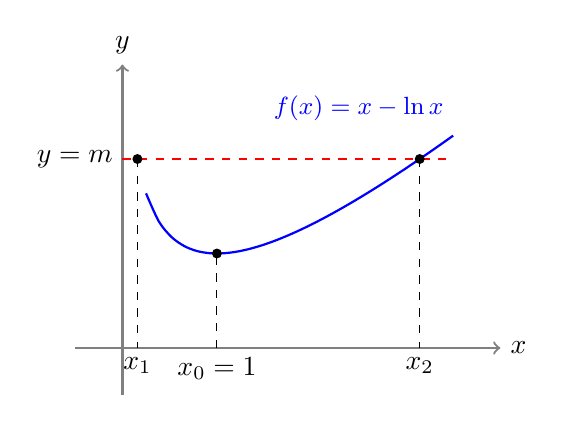
\begin{tikzpicture}[scale=1.2]
    % 坐标轴
    \draw[->, thick, gray] (-0.5, 0) -- (4, 0) node[right, black] {$x$};
    \draw[->, thick, gray] (0, -0.5) -- (0, 3) node[above, black] {$y$};
    
    % 函数 x - ln(x)
    \draw[domain=0.25:3.5, smooth, variable=\x, blue, thick] plot ({\x}, {\x - ln(\x)});
    
    % 极值点 x_0 = 1
    \draw[dashed] (1, 0) node[below] {$x_0=1$} -- (1, 1);
    \fill[black] (1, 1) circle (1.5pt);
    
    % 等高线 y = 2
    \def\m{2}
    \draw[dashed, red] (0, \m) node[left, black] {$y=m$} -- (3.5, \m);
    
    % 交点示意 
    \def\xone{0.1586}
    \def\xtwo{3.1462}
    \draw[dashed] (\xone, \m) -- (\xone, 0) node[below] {$x_1$};
    \draw[dashed] (\xtwo, \m) -- (\xtwo, 0) node[below] {$x_2$};
    
    \fill[black] (\xone, \m) circle (1.5pt);
    \fill[black] (\xtwo, \m) circle (1.5pt);
    
    \node[above, blue] at (2.5, 2.3) {\small $f(x)=x-\ln x$};
\end{tikzpicture}
\end{center}

\subsection{极值点偏移的本质图像与陡缓直觉}
假设函数 $f(x)$ 在 $x_0$ 处取极小值。水平线 $y=m$ 与函数图像交于两点 $x_1<x_0<x_2$，满足 $f(x_1)=f(x_2)=m$。
\begin{itemize}
    \item 如果图像两侧一样陡，那么 $x_1+x_2=2x_0$（严格对称，如 $x^2$）。
    \item 如果左边更陡，右边更缓，为了达到同样高度，右边要走得更远，于是 $x_2-x_0>x_0-x_1$，即 $x_1+x_2>2x_0$。
    \item 如果右边更陡，左边更缓，则 $x_1+x_2<2x_0$。
\end{itemize}
极值点偏移本质上就是：\textbf{两侧上升速度不同，导致等高点不再等距。}

\begin{keybox}{教师提示}
上面的说法是图像直觉，严格证明不能只靠“看图”，而要通过比较镜像点的函数值来完成。
\end{keybox}

\section{加法镜像：证明 $x_1+x_2>2$}
以 $x_0=1$ 为例，如果我们想判断 $x_1+x_2$ 与 $2$ 的大小关系，不要直接算 $x_1+x_2$，而是先找 $x_1$ 关于 $1$ 的\textbf{加法假想对称点}：
\[
x_1'=2-x_1
\]
设 $x_1=1-t$ ($0<t<1$)，则其加法镜像点为 $1+t$。
比较 $f(1-t)$ 与 $f(1+t)$ 的高度差异：
\[
f(1-t) = 1-t-\ln(1-t)
\]
\[
f(1+t) = 1+t-\ln(1+t)
\]
作差并设 $\varphi(t) = f(1-t)-f(1+t)$：
\[
\varphi(t) = \ln\frac{1+t}{1-t}-2t
\]
求导：
\[
\varphi'(t) = \frac{1}{1+t} + \frac{1}{1-t} - 2 = \frac{2}{1-t^2} - 2 = \frac{2t^2}{1-t^2} > 0
\]
又因为 $\varphi(0)=0$，所以当 $0<t<1$ 时，$\varphi(t)>0$，即 $f(1-t)>f(1+t)$。

这说明同样离极值点距离为 $t$，左边更高。由于右支是单调递增的，真正与 $x_1$ 等高的点 $x_2$ 必须比 $1+t$ 更靠右：
\[
x_2 > 1+t
\]
于是 $x_1+x_2 = (1-t) + x_2 > (1-t) + (1+t) = 2$。
结论得证：
\[
\boxed{x_1+x_2>2}
\]

\section{乘法镜像：证明 $x_1x_2<1$}
如果题目要求比较 $x_1x_2$ 与 $1$ 的关系，就不能再用加法对称点。要换一把尺子，用\textbf{乘法对称点}：
因为 $0<x_1<1$，它关于 $1$ 的乘法镜像点是 $\frac{1}{x_1}>1$。
比较 $f(1/x_1)$ 与 $f(x_1)$：
\[
f\left(\frac{1}{x_1}\right) - f(x_1) = \left(\frac{1}{x_1} - \ln\frac{1}{x_1}\right) - (x_1 - \ln x_1) = \frac{1}{x_1} - x_1 + 2\ln x_1
\]
构造函数 $\psi(x) = \frac{1}{x} - x + 2\ln x$ ($0<x<1$)。
求导：
\[
\psi'(x) = -\frac{1}{x^2} - 1 + \frac{2}{x} = -\frac{(x-1)^2}{x^2} < 0
\]
因为 $\psi'(x)<0$，且 $\psi(1)=0$，所以在 $(0,1)$ 上单调递减。这意味着当 $x$ 从 $x_1$ 增加到 $1$ 时，函数值逐渐下降，故必有：
\[
\psi(x_1)>\psi(1)=0.
\]
即 $f\left(\frac{1}{x_1}\right) > f(x_1)$。
又因为右支递增，而 $f(x_2)=f(x_1)$，所以真正的右侧等值点 $x_2$ 必须在 $\frac{1}{x_1}$ 的左边：
\[
x_2 < \frac{1}{x_1}
\]
由于 $x_1>0$，同乘 $x_1$ 得到：
\[
\boxed{x_1x_2<1}
\]

所以讲给学生的关键句是：
\[
\boxed{\text{看和，用加法镜像；看积，用乘法镜像。}}
\]

\section{教学与实战：如何破解极值点偏移？}

\begin{teachbox}{高中学生需要掌握到什么程度？}
对于普通高中学生，不需要把它学成一个很抽象的理论。真正要掌握的是下面四件事：
\begin{enumerate}
    \item \textbf{先看函数有没有单峰或单谷结构}：通过导数判断极值点，知道函数在极值点两侧分别单调。这是所有偏移题的基础。
    \item \textbf{知道等值点一定分布在极值点两侧}：很多学生一上来算 $x_1+x_2$ 或 $x_1x_2$，没有先确定它们在极值点两侧，后面就容易乱。
    \item \textbf{会判断“哪一侧更陡，哪一侧更缓”}：例如对 $f(x)=x-\ln x$，比较同距离点 $f(1-t)$ 和 $f(1+t)$。如果证明 $f(1-t)>f(1+t)$，说明左边更陡、右边更缓，于是等值点必然向右偏 $x_1+x_2>2$。
    \item \textbf{会选择“和偏移”还是“积偏移”}：对于正数函数经常隐藏着 $\ln x$ 变量。积关系本质上就是对数变量里的和关系：$x_1x_2=1 \Longleftrightarrow \ln x_1+\ln x_2=0$。例如 $x+\frac{1}{x}$ 应该看积，而 $x-\ln x$ 既可以看和偏移也可以看积偏移。
\end{enumerate}
\end{teachbox}

\begin{teachbox}{这节课最应该板书的主线}
可以直接这样板书，理清所有的思路盲点：
\begin{enumerate}
    \item \textbf{找极值点} $x_0$；
    \item \textbf{确认两侧单调}，等值点分居两侧；
    \item \textbf{看目标}：比较和还是积；
    \item \textbf{构造假想镜像点}；
    \item \textbf{比较镜像点与原点的函数值}；
    \item \textbf{用单调性推出真实等值点偏向哪边}。
\end{enumerate}
\end{teachbox}

\section{极值点偏移的三种层次}

\begin{teachbox}{三种对称尺度}
极值点偏移题的本质，不是机械判断 $x_1+x_2$ 或 $x_1x_2$，而是先判断函数在哪一种尺度下接近对称。

\begin{enumerate}
    \item \textbf{加法尺度}：围绕 $x_0$ 比较 $x_0-t$ 与 $x_0+t$，适合证明 $x_1+x_2$ 的偏移。
    \item \textbf{乘法尺度}：围绕 $x_0$ 比较 $x$ 与 $\frac{x_0^2}{x}$，适合证明 $x_1x_2$ 的偏移。
    \item \textbf{换元尺度}：通过 $u=\ln x$、$u=e^x$、$u=x^a$ 等变量代换，将陌生函数化成 $u-\ln u$ 或 $u+\frac1u$。
\end{enumerate}
\end{teachbox}

\section{和积互化：$\ln P = S - 2m$}
对于 $f(x)=x-\ln x$ ($x>0$)，若 $x_1<1<x_2$ 且 $f(x_1)=f(x_2)=m$ ($m>1$)。
由 $x_i-\ln x_i=m$ 得到 $\ln x_i=x_i-m$。两式相加：
\[
\ln x_1+\ln x_2 = x_1+x_2-2m
\]
令 $S=x_1+x_2$，$P=x_1x_2$，得到核心转化枢纽：
\[
\boxed{\ln P=S-2m} \quad \text{也就是} \quad \boxed{P=e^{S-2m}},\qquad \boxed{S=2m+\ln P}
\]
由此可以实现待证式的自由互化：
\[
\boxed{S>A \Longleftrightarrow P>e^{A-2m}} \quad \text{与} \quad \boxed{P>B \Longleftrightarrow S>2m+\ln B}
\]

\begin{keybox}{使用边界提醒}
注意，这里 $P=x_1x_2>0$，所以可以安全地对两边取对数；反过来，当从 $P>B$ 推出 $S>2m+\ln B$ 时，必须保证 $B>0$。
\end{keybox}

\section{增强函数法核心定理}

\begin{theorem}[和模型的增强函数法]
设 $f(x)=x-\ln x$，$m>1$，且 $x_1<1<x_2$ 满足
\[
f(x_1)=f(x_2)=m.
\]
记 $S=x_1+x_2$。对任意函数 $h$，令
\[
F_A(x)=x^2-Ax+h(f(x)).
\]
则有：
\[
F_A(x_2)-F_A(x_1)=(x_2-x_1)(S-A).
\]
因此，由于 $x_2-x_1>0$：
\[
S>A \Longleftrightarrow F_A(x_2)>F_A(x_1),
\]
\[
S<A \Longleftrightarrow F_A(x_2)<F_A(x_1).
\]
\end{theorem}

\begin{proof}
考虑 $g_A(x)=x^2-Ax$。作差有：
\[
g_A(x_2)-g_A(x_1) = x_2^2-x_1^2-A(x_2-x_1) = (x_2-x_1)(x_1+x_2-A) = (x_2-x_1)(S-A).
\]
因为 $f(x_1)=f(x_2)=m$，所以 $h(f(x_1))=h(f(x_2))=h(m)$。
于是：
\[
F_A(x_2)-F_A(x_1) = [g_A(x_2)+h(f(x_2))] - [g_A(x_1)+h(f(x_1))] = g_A(x_2)-g_A(x_1) = (x_2-x_1)(S-A).
\]
又因 $x_2-x_1>0$，故等价关系成立。
\end{proof}

\begin{theorem}[积模型的增强函数法]
设 $f(x)=x-\ln x$，$m>1$，且 $x_1<1<x_2$ 满足
\[
f(x_1)=f(x_2)=m.
\]
记 $P=x_1x_2$。对任意函数 $h$，令
\[
G_B(x)=x+\frac{B}{x}+h(f(x)).
\]
则有：
\[
G_B(x_2)-G_B(x_1)=(x_2-x_1)\left(1-\frac{B}{P}\right).
\]
因此，由于 $x_2-x_1>0$：
\[
P>B \Longleftrightarrow G_B(x_2)>G_B(x_1),
\]
\[
P<B \Longleftrightarrow G_B(x_2)<G_B(x_1).
\]
\end{theorem}

\begin{proof}
考虑 $g_B(x)=x+\frac{B}{x}$。作差有：
\[
g_B(x_2)-g_B(x_1) = x_2-x_1 + B\left(\frac{1}{x_2}-\frac{1}{x_1}\right) = (x_2-x_1) - B\frac{x_2-x_1}{x_1x_2} = (x_2-x_1)\left(1-\frac{B}{P}\right).
\]
因为 $h(f(x_1))=h(f(x_2))$，故：
\[
G_B(x_2)-G_B(x_1) = g_B(x_2)-g_B(x_1) = (x_2-x_1)\left(1-\frac{B}{P}\right).
\]
又因 $x_2-x_1>0$，故等价关系成立。
\end{proof}

\begin{teachbox}{增强函数法的思想本质}
已知 $f(x_1)=f(x_2)$，所以凡是只依赖于 $f(x)$ 的补偿项，在 $x_1,x_2$ 两端的取值相同，加入后不会改变端点差。

因此我们可以把一个原本不好比较的函数 $g(x)$，增强为
\[
F(x)=g(x)+h(f(x)),
\]
通过选择合适的 $h$，让 $F$ 的单调性、符号或导数结构变得更容易判断。

这不是为了“硬凑函数”，而是为了把目标不等式转化成端点比较。
\end{teachbox}

\section{母模型体系与结论推广的证明}

\subsection{$x-\ln x$}
这是最典型的“非对称极小值模型”。
基础结论：$\boxed{x_1+x_2>2}$，$\boxed{x_1x_2<1}$。（证明已在第三、四节给出）。

\subsection{$x+\frac{1}{x}$}
这是“严格乘法对称模型”。若 $x_1+\frac{1}{x_1}=x_2+\frac{1}{x_2}=m$（$0<x_1<1<x_2$），它不是“非对称偏移”，而是“乘法镜像的严格对称”。
\begin{proof}
移项有：
\[
x_2-x_1 = \frac{1}{x_1}-\frac{1}{x_2} = \frac{x_2-x_1}{x_1x_2}.
\]
因为 $x_2-x_1>0$，两边除以 $x_2-x_1$ 得到 $1 = \frac{1}{x_1x_2}$，即 $\boxed{x_1x_2=1}$。
再代回原等式 $x_1 + \frac{1}{x_1} = m$，利用 $\frac{1}{x_1}=x_2$，直接得到 $\boxed{x_1+x_2=m}$。
\end{proof}

\begin{center}
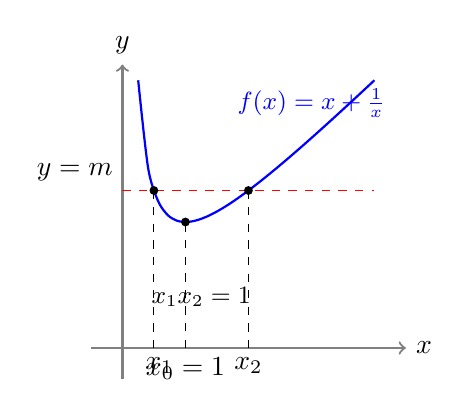
\begin{tikzpicture}[scale=0.8]
    % 坐标轴
    \draw[->, thick, gray] (-0.5, 0) -- (4.5, 0) node[right, black] {$x$};
    \draw[->, thick, gray] (0, -0.5) -- (0, 4.5) node[above, black] {$y$};
    
    % 函数 x + 1/x 在第一象限的图像
    \draw[domain=0.25:4, smooth, variable=\x, blue, thick] plot ({\x}, {\x + 1/\x});
    
    % 极小值点 x=1, y=2
    \draw[dashed] (1, 0) node[below] {$x_0=1$} -- (1, 2);
    \fill[black] (1, 2) circle (2pt);
    
    % 等高线 y = 2.5
    \def\m{2.5}
    \draw[dashed, red] (0, \m) node[above left, black] {$y=m$} -- (4, \m);
    
    % 交点 x=0.5, x=2
    \def\xone{0.5}
    \def\xtwo{2}
    \draw[dashed] (\xone, \m) -- (\xone, 0) node[below, xshift=2pt] {$x_1$};
    \draw[dashed] (\xtwo, \m) -- (\xtwo, 0) node[below] {$x_2$};
    
    \fill[black] (\xone, \m) circle (2pt);
    \fill[black] (\xtwo, \m) circle (2pt);
    
    \node[above, blue] at (3, 3.5) {\small $f(x)=x+\frac{1}{x}$};
    \node[above] at (1.25, 0.5) {\small $x_1 x_2 = 1$};
\end{tikzpicture}
\end{center}

\subsection{$\ln x+\frac{1}{x}$}
\begin{proof}
设 $F(x) = \ln x + \frac{1}{x}$。令 $u=\frac{1}{x}$，则 $\ln x = -\ln u$，所以有 $F(x) = u - \ln u$。
若 $x_1 < 1 < x_2$，则有 $u_1 = \frac{1}{x_1} > 1$，且 $u_2 = \frac{1}{x_2} < 1$。
在 $u$ 变量下，两个等值点分布在 $u_2 < 1 < u_1$。
由母模型 $u-\ln u$ 的结论直接可得：
\[
u_1+u_2>2,\qquad u_1u_2<1.
\]
代回 $x$ 的关系：
\[
\frac{1}{x_1}+\frac{1}{x_2}>2.
\]
而 $u_1u_2 = \frac{1}{x_1x_2} < 1 \implies \boxed{x_1x_2>1}$。
结论得证：$\boxed{\frac{1}{x_1}+\frac{1}{x_2}>2}$ 且 $\boxed{x_1x_2>1}$。

\textbf{注意}：此处应提醒学生，不要直接把 $x-\ln x$ 的常数结论机械照搬，而是先换元到 $u$，再翻译回来。
\end{proof}

\subsection{$x^a-a\ln x$}
对 $f(x)=x^a-a\ln x$ （其中 $a>0$, $x>0$）。
\begin{proof}
令 $u=x^a$，则 $\ln u = a\ln x$，所以 $f(x) = u - \ln u$。
若 $f(x_1) = f(x_2)$，则 $u_1-\ln u_1 = u_2-\ln u_2$，其中 $u_1=x_1^a$, $u_2=x_2^a$。
因为 $a>0$，幂函数 $x^a$ 单调递增，所以 $x_1 < 1 < x_2 \Longleftrightarrow u_1 < 1 < u_2$。
由母模型结论有 $u_1+u_2 > 2$ 且 $u_1u_2 < 1$。
翻译回原变量即得：$\boxed{x_1^a+x_2^a>2}$ 且 $x_1^ax_2^a < 1$。因 $a>0$，则 $(x_1x_2)^a < 1 \Longleftrightarrow \boxed{x_1x_2<1}$。
\end{proof}

\subsection{$xe^{-x}$ 与 $x^ae^{-bx}$}
设 $f(x)=xe^{-x}$ ($x>0$)。极值点在 $x=1$。若 $x_1e^{-x_1}=x_2e^{-x_2}=c$ ($0<c<1/e$)，且 $0<x_1<1<x_2$。
\begin{proof}
两边取对数得：$\ln x_1 - x_1 = \ln x_2 - x_2 \implies x_1 - \ln x_1 = x_2 - \ln x_2$。
直接化为母模型 $x-\ln x$。故可直接得到：$\boxed{x_1+x_2>2}$，$\boxed{x_1x_2<1}$。
\end{proof}

\begin{center}
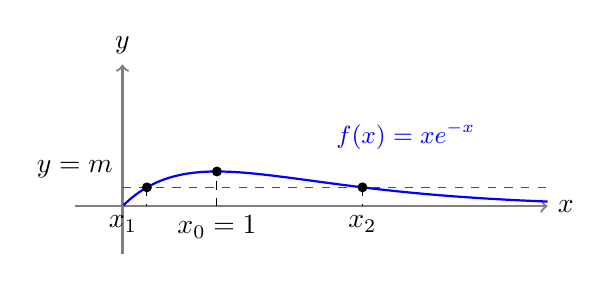
\begin{tikzpicture}[scale=1.2]
    % 坐标轴
    \draw[->, thick, gray] (-0.5, 0) -- (4.5, 0) node[right, black] {$x$};
    \draw[->, thick, gray] (0, -0.5) -- (0, 1.5) node[above, black] {$y$};
    
    % 函数 x e^{-x}
    \draw[domain=0.01:4.5, smooth, samples=100, variable=\x, blue, thick] plot ({\x}, {\x * exp(-\x)});
    
    % 极大值点 x=1, y=1/e ~ 0.368
    \draw[dashed] (1, 0) node[below] {$x_0=1$} -- (1, 0.368);
    \fill[black] (1, 0.368) circle (1.5pt);
    
    % 等高线 y=0.2
    \def\m{0.2}
    \draw[dashed, red] (0, \m) node[above left, black] {$y=m$} -- (4.5, \m);
    
    % 交点 x_1 ~ 0.259, x_2 ~ 2.54
    \def\xone{0.259}
    \def\xtwo{2.54}
    \draw[dashed] (\xone, \m) -- (\xone, 0) node[below left] {$x_1$};
    \draw[dashed] (\xtwo, \m) -- (\xtwo, 0) node[below] {$x_2$};
    
    \fill[black] (\xone, \m) circle (1.5pt);
    \fill[black] (\xtwo, \m) circle (1.5pt);
    
    \node[above, blue] at (3, 0.5) {\small $f(x)=x e^{-x}$};
\end{tikzpicture}
\end{center}

更一般地，对于 $x^ae^{-bx}$ （其中 $a>0, b>0, x>0$），其最大值点为 $x_0 = \frac{a}{b}$。等值点满足 $0 < x_1 < \frac{a}{b} < x_2$ 且 $x_1^ae^{-bx_1}=x_2^ae^{-bx_2}$。
\begin{proof}
两边取对数得：$a\ln x_1 - bx_1 = a\ln x_2 - bx_2 \implies bx_1 - a\ln x_1 = bx_2 - a\ln x_2$。
两边除以 $a$：
\[
\frac{b}{a}x_1 - \ln x_1 = \frac{b}{a}x_2 - \ln x_2.
\]
令 $u = \frac{b}{a}x$，则 $x = \frac{a}{b}u$, 且 $\ln x = \ln u + \ln\frac{a}{b}$。
代入得：
\[
u_1 - \ln u_1 - \ln\frac{a}{b} = u_2 - \ln u_2 - \ln\frac{a}{b} \implies u_1 - \ln u_1 = u_2 - \ln u_2.
\]
常数项消去不影响自变量大小比较，且因为 $0<x_1<\frac{a}{b}<x_2$，代入换元后满足 $0<u_1<1<u_2$。
由母模型结论有 $u_1+u_2>2$ 且 $u_1u_2<1$。
翻译回 $x$ 的关系：
\[
\frac{b}{a}x_1 + \frac{b}{a}x_2 > 2 \implies \boxed{x_1+x_2 > \frac{2a}{b}}.
\]
\[
\left(\frac{b}{a}x_1\right)\left(\frac{b}{a}x_2\right) < 1 \implies \frac{b^2}{a^2}x_1x_2 < 1 \implies \boxed{x_1x_2 < \left(\frac{a}{b}\right)^2}.
\]
此证明完整体现了“换元归化”的转化思想。
\end{proof}

\begin{teachbox}{母模型体系一览表}
\begin{center}
\renewcommand{\arraystretch}{1.4}
\setlength{\tabcolsep}{12pt}
\begin{tabular}{llll}
\toprule
\textbf{模型} & \textbf{变量代换} & \textbf{归化后模型} & \textbf{典型结论}\\
\midrule
$x-\ln x$ & $u=x$ & $u-\ln u$ & $x_1+x_2>2$, $x_1x_2<1$\\
$\ln x+\frac{1}{x}$ & $u=\frac{1}{x}$ & $u-\ln u$ & $\frac{1}{x_1}+\frac{1}{x_2}>2$, $x_1x_2>1$\\
$x^a-a\ln x$ & $u=x^a$ & $u-\ln u$ & $x_1^a+x_2^a>2$, $x_1x_2<1$\\
$xe^{-x}$ & 取对数 & $x-\ln x$ & $x_1+x_2>2$, $x_1x_2<1$\\
$x^ae^{-bx}$ & $u=\frac{b}{a}x$ & $u-\ln u$ & $x_1+x_2>\frac{2a}{b}$, $x_1x_2<\left(\frac{a}{b}\right)^2$\\
\bottomrule
\end{tabular}
\end{center}
\end{teachbox}

\begin{keybox}{参数与定义域提醒}
下表中的函数均需在相应定义域和参数条件下讨论。例如 $x-a\ln x$ 默认 $a>0,x>0$；$x+\frac ax$ 默认 $a>0,x>0$；$x^ae^{-bx}$ 默认 $a>0,b>0,x>0$；涉及 $x^p$ 的模型默认在正数范围内讨论。
\end{keybox}

\begin{keybox}{使用说明}
下表不是学生背诵清单，而是教师备课时用于识别母模型的索引。遇到陌生函数时，先考虑取对数、换元、平移、缩放，而不是直接套表。
\end{keybox}

\section{经典函数清单大字典}

除了上述几大核心母模型，高考和竞赛中经常会通过各种形式隐藏极值点模型。下面列出常考的 $17$ 种经典函数，作为教师备课的大字典：

\begin{center}
\renewcommand{\arraystretch}{1.4}
\setlength{\tabcolsep}{22pt}
\begin{longtable}{llll}
\toprule
\textbf{类型} & \textbf{经典函数} & \textbf{极值点} & \textbf{本质母模型} \\
\midrule
对数线性型 & $x-\ln x$ & $1$ & $u-\ln u$ \\
对数线性型 & $x-a\ln x$ & $a$ & $u-\ln u$ \\
对数线性型 & $x^p-p\ln x$ & $1$ & $u-\ln u$ \\
平移对数型 & $x-\ln(1+x)$ & $0$ & $u-\ln u$ \\
指数线性型 & $e^x-x$ & $0$ & $u-\ln u$ \\
对数倒数型 & $\ln x+\frac{1}{x}$ & $1$ & $u-\ln u$ \\
倒数型 & $x+\frac{1}{x}$ & $1$ & $u+\frac{1}{u}$ \\
倒数型 & $x+\frac{a}{x}$ & $\sqrt{a}$ & $u+\frac{1}{u}$ \\
幂倒数型 & $x^p+x^{-p}$ & $1$ & $u+\frac{1}{u}$ \\
指数对称型 & $e^x+e^{-x}$ & $0$ & $u+\frac{1}{u}$ \\
指数对称型 & $ae^{kx}+be^{-kx}$ & $\frac{1}{2k}\ln\frac{b}{a}$ & $u+\frac{1}{u}$ \\
指数衰减型 & $xe^{-x}$ & $1$ & $ue^{-u}$ \\
Gamma 型 & $x^ae^{-bx}$ & $\frac{a}{b}$ & $ue^{-u}$ \\
对数商型 & $\frac{\ln x}{x}$ & $e$ & $ue^{-u}$ \\
幂指数型 & $x^{1/x}$ & $e$ & $\frac{\ln x}{x}$ \\
熵函数型 & $x\ln x$ & $\frac{1}{e}$ & $ue^{-u}$ \\
幂幂型 & $x^x$ & $\frac{1}{e}$ & $x\ln x$ \\
\bottomrule
\end{longtable}
\end{center}

\section{进阶：$S=x_1+x_2$ 的精细估计}

\begin{keybox}{教师提示与分层教学口径}
本节属于教师备课与尖子生探究内容。普通学生（非竞赛/非强基）不要求掌握双曲函数参数化分析方法。以下精细估计不是学生强记硬背的内容，而是作为展示“如何由母模型生成与验证更强的不等式”的教研与培优材料。
\end{keybox}

设 $m>1$，$x_1<1<x_2$ 为方程 $x-\ln x=m$ 的两根，记 $S=x_1+x_2$, $P=x_1x_2$。

\subsection{基础强下界：$S>m$}
因为 $x_2-\ln x_2=m$，且 $x_2>1$，所以 $\ln x_2>0$，从而有：
\[
x_2=m+\ln x_2>m.
\]
故：
\[
S=x_1+x_2>x_2>m.
\]
此不等式比常数界 $S>2$ 在 $m$ 较大时要强得多。由于 $S>m > m-1$，故 $S>m-1$ 也自然成立。

\subsection{统一参数化工具}
两式相减有：
\[
x_2-x_1=\ln x_2-\ln x_1 = \ln\frac{x_2}{x_1}.
\]
令 $x_2-x_1=2t$ ($t>0$)，则 $\ln\frac{x_2}{x_1}=2t \implies \frac{x_2}{x_1}=e^{2t}$。
结合差值有 $e^{2t}x_1-x_1=2t \implies x_1=\frac{2t}{e^{2t}-1} = \frac{t e^{-t}}{\sinh t}$。
同理可得 $x_2=\frac{te^t}{\sinh t}$。
由此，和 $S$ 与高度 $m$ 都可以用单变量 $t$ 统一转化为关于 $t$ 的单变量不等式来表示：
\[
S=x_1+x_2 = 2t\coth t.
\]
\[
2m = S - \ln P = 2t\coth t - \ln\left(\frac{t^2}{\sinh^2 t}\right) \implies m = t\coth t + \ln\frac{\sinh t}{t}.
\]
令 $C=t\coth t$，$L=\ln\frac{\sinh t}{t}$，则有：
\[
\boxed{S=2C} \qquad \boxed{m=C+L}.
\]
这套工具能把所有关于 $S, m$ 的复杂估计不等式，统一转化为关于 $t$ 的单变量不等式进行严格验证。

\subsection{代表性上界：$S<\frac{4m+2}{3}$}
要证 $S<\frac{4m+2}{3}$，代入参数化工具等价于证明：
\[
2C < \frac{4(C+L)+2}{3} \Longleftrightarrow 6C < 4C+4L+2 \Longleftrightarrow C < 2L+1.
\]
即证明：
\[
t\coth t < 1 + 2\ln\frac{\sinh t}{t}.
\]
\begin{proof}
令
\[
R(t)=1+2\ln\frac{\sinh t}{t}-t\coth t.
\]
显然
\[
\lim_{t\to0^+}R(t)=0.
\]
求导得
\[
R'(t)
=
2\left(\coth t-\frac1t\right)
-
\left(\coth t-t\csch^2t\right)
=
\coth t-\frac2t+t\csch^2t.
\]
由于
\[
t\sinh^2t>0,
\]
所以 $R'(t)>0$ 等价于
\[
t\sinh t\cosh t-2\sinh^2t+t^2>0.
\]
记
\[
K(t)=t\sinh t\cosh t-2\sinh^2t+t^2.
\]
下面严格证明 $K(t)>0$。

利用恒等式
\[
\sinh t\cosh t=\frac12\sinh 2t,
\qquad
2\sinh^2t=\cosh 2t-1,
\]
可得
\[
K(t)
=
\frac t2\sinh 2t-\cosh 2t+1+t^2.
\]
展开幂级数：
\[
\frac t2\sinh 2t
=
\sum_{n=1}^{\infty}
\frac{2^{2n-2}}{(2n-1)!}t^{2n},
\]
\[
\cosh 2t
=
\sum_{n=0}^{\infty}
\frac{2^{2n}}{(2n)!}t^{2n}.
\]
代入 $K(t)$ 后，常数项、$t^2$ 项与 $t^4$ 项全部抵消。对 $n\ge3$，$t^{2n}$ 的系数为
\[
\frac{2^{2n-2}}{(2n-1)!}
-
\frac{2^{2n}}{(2n)!}
=
\frac{2^{2n-2}}{(2n-1)!}
\left(1-\frac{4}{2n}\right)
=
\frac{2^{2n-2}(n-2)}{n(2n-1)!}.
\]
因此
\[
K(t)
=
\sum_{n=3}^{\infty}
\frac{2^{2n-2}(n-2)}{n(2n-1)!}t^{2n}.
\]
当 $t>0$ 时，右侧每一项均为正，所以
\[
K(t)>0.
\]
于是
\[
R'(t)>0.
\]
又因为 $\lim_{t\to0^+}R(t)=0$，且 $R'(t)>0$，所以当 $t>0$ 时恒有 $R(t)>0$。
即
\[
t\coth t<1+2\ln\frac{\sinh t}{t},
\]
也就是
\[
C<2L+1.
\]
于是
\[
S=2C
<
\frac{4(C+L)+2}{3}
=
\frac{4m+2}{3}.
\]
故
\[
\boxed{S<\frac{4m+2}{3}}.
\]
\end{proof}

\subsection{由强下界推出弱下界：$S > \frac{2}{3}m - \frac{4}{3}\sqrt{m}$}
\begin{proof}
由第一节及 11.1 已严格证明的基础强下界 $S > m$。
我们只需考察 $m$ 与目标下界的关系。作差：
\[
m - \left( \frac{2}{3}m - \frac{4}{3}\sqrt{m} \right) = \frac{1}{3}m + \frac{4}{3}\sqrt{m} > 0 \quad (\text{因 } m>1).
\]
因此，在 $m>1$ 时有 $m > \frac{2}{3}m - \frac{4}{3}\sqrt{m}$。
结合已证的 $S>m$，立刻有：
\[
S > m > \frac{2}{3}m - \frac{4}{3}\sqrt{m}.
\]
\textbf{注意}：此处应提醒学生，这不是一个新的深界，而是由基础强下界 $S>m$ 直接推出的弱界推论。
\end{proof}

\begin{keybox}{教师备查：根号上界}
还可以证明：
\[
S<m+\sqrt{m}.
\]
利用参数化表示为 $C-L < \sqrt{C+L}$，即证明：
\[
H_1(t)=C+L-(C-L)^2>0.
\]
该正性可以通过对单变量函数 $H_1(t)$ 的进一步导数求导与单调性分析证明，但化简过程较长，不作为本讲义正文重点。
\end{keybox}

\begin{keybox}{教师备查：对数下界}
还可以证明：
\[
S > m + \frac{1}{m} + \ln m.
\]
利用参数化表示为 $C-L > \frac{1}{C+L} + \ln(C+L)$，即证明：
\[
H_2(t)=C-L-\frac{1}{C+L}-\ln(C+L)>0.
\]
注意：此处不能简单写作 $H_2'(t)>0$，因为 $H_2'(t)$ 并非在整个 $(0,+\infty)$ 上恒正（在大 $t$ 时其导数会变为负数）。若要严格证明此结论，需要作分段精细放缩或局部正性分析。
\end{keybox}

\begin{keybox}{教师备查：对数上界}
还可以证明：
\[
S < m + \frac{m\ln m}{m-1}.
\]
利用参数化表示为 $C-L < \frac{(C+L)\ln(C+L)}{C+L-1}$，即证明：
\[
H_3(t)=\frac{(C+L)\ln(C+L)}{C+L-1}-(C-L)>0.
\]
该结论同样需要对 $H_3(t)$ 作较长的单变量函数讨论，在常规教学中作为结论性结论备查即可。
\end{keybox}

\subsection{估计结论的跨模型迁移与应用}
凡是在母模型 $u-\ln u=m$ 中已经严格证明的估计结论，都可以通过换元无缝迁移到其他非对称模型中。这正是“母模型体系”的核心威力。

\textbf{迁移例 1：指数衰减模型 $xe^{-x}$}
设 $0<x_1<1<x_2$ 满足 $x_1e^{-x_1} = x_2e^{-x_2} = c$。取对数并移项有 $x_i - \ln x_i = -\ln c$。
令极小值高度 $m = -\ln c > 1$，对于已在母模型中严格证明的结论，直接套用可得：
\begin{itemize}
    \item 基础下界：$x_1+x_2 > -\ln c$
    \item 线性上界：$x_1+x_2 < \frac{-4\ln c + 2}{3}$
\end{itemize}

\textbf{迁移例 2：对数倒数模型 $\ln x + 1/x$}
设 $x_1 < 1 < x_2$ 满足 $\ln x_1 + \frac{1}{x_1} = \ln x_2 + \frac{1}{x_2} = m$。
令 $u = \frac{1}{x}$，则归化为 $u - \ln u = m$，其中 $u_2 < 1 < u_1$。
直接套用已证的 $u_1+u_2$ 即 $\frac{1}{x_1} + \frac{1}{x_2}$ 的估计结论：
\begin{itemize}
    \item 基础下界：$\frac{1}{x_1} + \frac{1}{x_2} > m$
    \item 线性上界：$\frac{1}{x_1} + \frac{1}{x_2} < \frac{4m+2}{3}$
\end{itemize}
通过这种“定理—证明—迁移”的结构，学生不仅掌握了具体的数学不等式，更深刻体会到了通过换元将复杂未知转化为已知母模型的代数同构思想。

\end{document}
